\documentclass[twoside]{book}

% Packages required by doxygen
\usepackage{fixltx2e}
\usepackage{calc}
\usepackage{doxygen}
\usepackage[export]{adjustbox} % also loads graphicx
\usepackage{graphicx}
\usepackage[utf8]{inputenc}
\usepackage{makeidx}
\usepackage{multicol}
\usepackage{multirow}
\PassOptionsToPackage{warn}{textcomp}
\usepackage{textcomp}
\usepackage[nointegrals]{wasysym}
\usepackage[table]{xcolor}

% Font selection
\usepackage[T1]{fontenc}
\usepackage[scaled=.90]{helvet}
\usepackage{courier}
\usepackage{amssymb}
\usepackage{sectsty}
\renewcommand{\familydefault}{\sfdefault}
\allsectionsfont{%
  \fontseries{bc}\selectfont%
  \color{darkgray}%
}
\renewcommand{\DoxyLabelFont}{%
  \fontseries{bc}\selectfont%
  \color{darkgray}%
}
\newcommand{\+}{\discretionary{\mbox{\scriptsize$\hookleftarrow$}}{}{}}

% Page & text layout
\usepackage{geometry}
\geometry{%
  a4paper,%
  top=2.5cm,%
  bottom=2.5cm,%
  left=2.5cm,%
  right=2.5cm%
}
\tolerance=750
\hfuzz=15pt
\hbadness=750
\setlength{\emergencystretch}{15pt}
\setlength{\parindent}{0cm}
\setlength{\parskip}{3ex plus 2ex minus 2ex}
\makeatletter
\renewcommand{\paragraph}{%
  \@startsection{paragraph}{4}{0ex}{-1.0ex}{1.0ex}{%
    \normalfont\normalsize\bfseries\SS@parafont%
  }%
}
\renewcommand{\subparagraph}{%
  \@startsection{subparagraph}{5}{0ex}{-1.0ex}{1.0ex}{%
    \normalfont\normalsize\bfseries\SS@subparafont%
  }%
}
\makeatother

% Headers & footers
\usepackage{fancyhdr}
\pagestyle{fancyplain}
\fancyhead[LE]{\fancyplain{}{\bfseries\thepage}}
\fancyhead[CE]{\fancyplain{}{}}
\fancyhead[RE]{\fancyplain{}{\bfseries\leftmark}}
\fancyhead[LO]{\fancyplain{}{\bfseries\rightmark}}
\fancyhead[CO]{\fancyplain{}{}}
\fancyhead[RO]{\fancyplain{}{\bfseries\thepage}}
\fancyfoot[LE]{\fancyplain{}{}}
\fancyfoot[CE]{\fancyplain{}{}}
\fancyfoot[RE]{\fancyplain{}{\bfseries\scriptsize Generated by Doxygen }}
\fancyfoot[LO]{\fancyplain{}{\bfseries\scriptsize Generated by Doxygen }}
\fancyfoot[CO]{\fancyplain{}{}}
\fancyfoot[RO]{\fancyplain{}{}}
\renewcommand{\footrulewidth}{0.4pt}
\renewcommand{\chaptermark}[1]{%
  \markboth{#1}{}%
}
\renewcommand{\sectionmark}[1]{%
  \markright{\thesection\ #1}%
}

% Indices & bibliography
\usepackage{natbib}
\usepackage[titles]{tocloft}
\setcounter{tocdepth}{3}
\setcounter{secnumdepth}{5}
\makeindex

% Hyperlinks (required, but should be loaded last)
\usepackage{ifpdf}
\ifpdf
  \usepackage[pdftex,pagebackref=true]{hyperref}
\else
  \usepackage[ps2pdf,pagebackref=true]{hyperref}
\fi
\hypersetup{%
  colorlinks=true,%
  linkcolor=blue,%
  citecolor=blue,%
  unicode%
}

% Custom commands
\newcommand{\clearemptydoublepage}{%
  \newpage{\pagestyle{empty}\cleardoublepage}%
}

\usepackage{caption}
\captionsetup{labelsep=space,justification=centering,font={bf},singlelinecheck=off,skip=4pt,position=top}

%===== C O N T E N T S =====

\begin{document}

% Titlepage & ToC
\hypersetup{pageanchor=false,
             bookmarksnumbered=true,
             pdfencoding=unicode
            }
\pagenumbering{alph}
\begin{titlepage}
\vspace*{7cm}
\begin{center}%
{\Large Square\+Eq\+Solver \\[1ex]\large 1.\+0 }\\
\vspace*{1cm}
{\large Generated by Doxygen 1.8.13}\\
\end{center}
\end{titlepage}
\clearemptydoublepage
\pagenumbering{roman}
\tableofcontents
\clearemptydoublepage
\pagenumbering{arabic}
\hypersetup{pageanchor=true}

%--- Begin generated contents ---
\chapter{Todo List}
\label{todo}
\Hypertarget{todo}

\begin{DoxyRefList}
\item[\label{todo__todo000001}%
\Hypertarget{todo__todo000001}%
File \hyperlink{main_8cpp}{main.cpp} ]Ругается на N\+AN, ругается на сравнение с нулем, дописать нахождение комплексных корней, почему не комментируются переменные? 
\end{DoxyRefList}
\chapter{File Index}
\section{File List}
Here is a list of all documented files with brief descriptions\+:\begin{DoxyCompactList}
\item\contentsline{section}{/home/filipphristolubov/\+Square\+Eq\+Solver\+\_\+1\+\_\+0/\hyperlink{main_8cpp}{main.\+cpp} \\*Первое домашнее задание по курсу \char`\"{}Введение в промышленное программирование и структуры данных\char`\"{} }{\pageref{main_8cpp}}{}
\end{DoxyCompactList}

\chapter{File Documentation}
\hypertarget{main_8cpp}{}\section{/home/filipphristolubov/\+Square\+Eq\+Solver\+\_\+1\+\_\+0/main.cpp File Reference}
\label{main_8cpp}\index{/home/filipphristolubov/\+Square\+Eq\+Solver\+\_\+1\+\_\+0/main.\+cpp@{/home/filipphristolubov/\+Square\+Eq\+Solver\+\_\+1\+\_\+0/main.\+cpp}}


Первое домашнее задание по курсу \char`\"{}Введение в промышленное программирование и структуры данных\char`\"{}.  


{\ttfamily \#include $<$stdio.\+h$>$}\newline
{\ttfamily \#include $<$math.\+h$>$}\newline
{\ttfamily \#include $<$cassert$>$}\newline
Include dependency graph for main.\+cpp\+:
\nopagebreak
\begin{figure}[H]
\begin{center}
\leavevmode
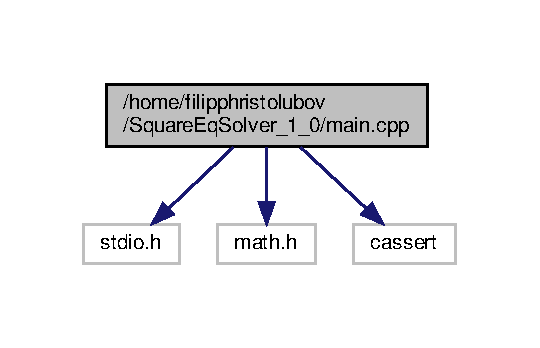
\includegraphics[width=259pt]{main_8cpp__incl}
\end{center}
\end{figure}
\subsection*{Macros}
\begin{DoxyCompactItemize}
\item 
\mbox{\Hypertarget{main_8cpp_aeca034f67218340ecb2261a22c2f3dcd}\label{main_8cpp_aeca034f67218340ecb2261a22c2f3dcd}} 
\#define \hyperlink{main_8cpp_aeca034f67218340ecb2261a22c2f3dcd}{B\+U\+F\+S\+I\+ZE}~100
\begin{DoxyCompactList}\small\item\em difines the size of buffer for user input \end{DoxyCompactList}\item 
\mbox{\Hypertarget{main_8cpp_a270b1ecf56619755ce62f6970dfabc91}\label{main_8cpp_a270b1ecf56619755ce62f6970dfabc91}} 
\#define \hyperlink{main_8cpp_a270b1ecf56619755ce62f6970dfabc91}{e}~1e-\/14
\begin{DoxyCompactList}\small\item\em if module of value less than e, we consider it to be 0 \end{DoxyCompactList}\item 
\mbox{\Hypertarget{main_8cpp_a0d8ff9279a45a14f1f7f0d2682b43bfb}\label{main_8cpp_a0d8ff9279a45a14f1f7f0d2682b43bfb}} 
\#define \hyperlink{main_8cpp_a0d8ff9279a45a14f1f7f0d2682b43bfb}{zero\+\_\+check}(inp)~((inp $>$ -\/\hyperlink{main_8cpp_a270b1ecf56619755ce62f6970dfabc91}{e}) \&\& (inp $<$ \hyperlink{main_8cpp_a270b1ecf56619755ce62f6970dfabc91}{e}) ? 0 \+: inp)
\begin{DoxyCompactList}\small\item\em chek if module of value is less than e, end if yes, equate it to 0 \end{DoxyCompactList}\end{DoxyCompactItemize}
\subsection*{Enumerations}
\begin{DoxyCompactItemize}
\item 
\mbox{\Hypertarget{main_8cpp_a06fc87d81c62e9abb8790b6e5713c55b}\label{main_8cpp_a06fc87d81c62e9abb8790b6e5713c55b}} 
enum \{ {\bfseries C\+O\+M\+P\+L\+E\+X\+\_\+\+R\+O\+O\+TS} = -\/1, 
{\bfseries N\+O\+\_\+\+R\+O\+O\+TS}, 
{\bfseries O\+N\+E\+\_\+\+R\+O\+OT}, 
{\bfseries T\+W\+O\+\_\+\+R\+O\+O\+TS}
 \}
\end{DoxyCompactItemize}
\subsection*{Functions}
\begin{DoxyCompactItemize}
\item 
int \hyperlink{main_8cpp_a24e8c4330e2f981993e801bb957193a6}{Solve\+Linear} (double b, double c, double $\ast$x1)
\begin{DoxyCompactList}\small\item\em Solves bx+c=0 linear equation. \end{DoxyCompactList}\item 
int \hyperlink{main_8cpp_aeab310e5c94ddb7783b52251c9eb79aa}{Solve\+Sqare} (double a, double b, double c, double $\ast$x1, double $\ast$x2)
\begin{DoxyCompactList}\small\item\em Solves ax$^\wedge$2+bx+c=0 equation. \end{DoxyCompactList}\item 
int \hyperlink{main_8cpp_ae66f6b31b5ad750f1fe042a706a4e3d4}{main} ()
\end{DoxyCompactItemize}


\subsection{Detailed Description}
Первое домашнее задание по курсу \char`\"{}Введение в промышленное программирование и структуры данных\char`\"{}. 

\begin{DoxyAuthor}{Author}
Philip Khristolyubov 
\end{DoxyAuthor}
\begin{DoxyVersion}{Version}
1.\+0 
\end{DoxyVersion}
\begin{DoxyDate}{Date}
27.\+09.\+2018 
\end{DoxyDate}
\begin{DoxyRefDesc}{Todo}
\item[\hyperlink{todo__todo000001}{Todo}]Ругается на N\+AN, ругается на сравнение с нулем, дописать нахождение комплексных корней, почему не комментируются переменные? \end{DoxyRefDesc}


\subsection{Function Documentation}
\mbox{\Hypertarget{main_8cpp_ae66f6b31b5ad750f1fe042a706a4e3d4}\label{main_8cpp_ae66f6b31b5ad750f1fe042a706a4e3d4}} 
\index{main.\+cpp@{main.\+cpp}!main@{main}}
\index{main@{main}!main.\+cpp@{main.\+cpp}}
\subsubsection{\texorpdfstring{main()}{main()}}
{\footnotesize\ttfamily int main (\begin{DoxyParamCaption}{ }\end{DoxyParamCaption})}

$<$ \textquotesingle{}a\textquotesingle{}, \textquotesingle{}b\textquotesingle{}, \textquotesingle{}c\textquotesingle{} coefficents of ax$^\wedge$2+bx+c equation

$<$ buffer for user input

$<$ first and second roots of the square equation \mbox{\Hypertarget{main_8cpp_a24e8c4330e2f981993e801bb957193a6}\label{main_8cpp_a24e8c4330e2f981993e801bb957193a6}} 
\index{main.\+cpp@{main.\+cpp}!Solve\+Linear@{Solve\+Linear}}
\index{Solve\+Linear@{Solve\+Linear}!main.\+cpp@{main.\+cpp}}
\subsubsection{\texorpdfstring{Solve\+Linear()}{SolveLinear()}}
{\footnotesize\ttfamily int Solve\+Linear (\begin{DoxyParamCaption}\item[{double}]{b,  }\item[{double}]{c,  }\item[{double $\ast$}]{x1 }\end{DoxyParamCaption})}



Solves bx+c=0 linear equation. 


\begin{DoxyParams}{Parameters}
{\em b\mbox{[}in\mbox{]}} & \textquotesingle{}b\textquotesingle{} coefficient of equation \\
\hline
{\em c\mbox{[}in\mbox{]}} & \textquotesingle{}c\textquotesingle{} coefficient of equation \\
\hline
{\em x1\mbox{[}out\mbox{]}} & pointer to the root of equation \\
\hline
\end{DoxyParams}
\begin{DoxyReturn}{Returns}
number of found roots 
\end{DoxyReturn}
\mbox{\Hypertarget{main_8cpp_aeab310e5c94ddb7783b52251c9eb79aa}\label{main_8cpp_aeab310e5c94ddb7783b52251c9eb79aa}} 
\index{main.\+cpp@{main.\+cpp}!Solve\+Sqare@{Solve\+Sqare}}
\index{Solve\+Sqare@{Solve\+Sqare}!main.\+cpp@{main.\+cpp}}
\subsubsection{\texorpdfstring{Solve\+Sqare()}{SolveSqare()}}
{\footnotesize\ttfamily int Solve\+Sqare (\begin{DoxyParamCaption}\item[{double}]{a,  }\item[{double}]{b,  }\item[{double}]{c,  }\item[{double $\ast$}]{x1,  }\item[{double $\ast$}]{x2 }\end{DoxyParamCaption})}



Solves ax$^\wedge$2+bx+c=0 equation. 


\begin{DoxyParams}{Parameters}
{\em a\mbox{[}in\mbox{]}} & \textquotesingle{}a\textquotesingle{} coefficient of equation \\
\hline
{\em b\mbox{[}in\mbox{]}} & \textquotesingle{}b\textquotesingle{} coefficient of equation \\
\hline
{\em c\mbox{[}in\mbox{]}} & \textquotesingle{}c\textquotesingle{} coefficient of equation \\
\hline
{\em x1\mbox{[}out\mbox{]}} & pointer to the first root of equation \\
\hline
{\em x2\mbox{[}out\mbox{]}} & pointer to the second root of equation \\
\hline
\end{DoxyParams}
\begin{DoxyReturn}{Returns}
number of found roots 
\end{DoxyReturn}
$<$ D discriminant of the equation $\ast$/ 
%--- End generated contents ---

% Index
\backmatter
\newpage
\phantomsection
\clearemptydoublepage
\addcontentsline{toc}{chapter}{Index}
\printindex

\end{document}
